%\documentclass{sig-alternate}
\documentclass[conference]{IEEEtran}

\usepackage{graphicx}
\usepackage{pifont}
\usepackage{url}
\usepackage{code}
\usepackage{amsmath}

\newcommand{\comment}[1]{}

\title{Reduce Before You Localize:  Delta-Debugging and Spectrum-Based Fault Localization}


\author{\IEEEauthorblockN{%
Arpit Christi,\IEEEauthorrefmark{1}
Matthew Lyle Olson,\IEEEauthorrefmark{1}
Mohammad Amin Alipour,\IEEEauthorrefmark{2}
Alex Groce\IEEEauthorrefmark{3}
}


\IEEEauthorblockA{\IEEEauthorrefmark{1}%
EECS, Oregon State University \{christia,olsonm\}@oregonstate.edu%
\\
\IEEEauthorrefmark{2}%
University of Houston alipour@cs.uh.edu%
\\
\IEEEauthorrefmark{3}%
SICCS, Northern Arizona University, agroce@gmail.com%
\\
}


%\author{\IEEEauthorblockN{Alex Groce, Amin Alipour, Chaoqiang Zhang, Yang Chen, John Regehr}
%\IEEEauthorblockA{School of Electrical Engineering and Computer Science\\
%Oregon State University, Corvallis, OR\\
%Email: agroce@gmail.com, alipourm,zhangch@onid.oregonstate.edu}}
}

\comment{
\numberofauthors{1}
\author{
\alignauthor
Arpit Christi, Matthew Lyle Olson, Mohammad Amin Alipour, Alex Groce\\
\affaddr{School of Electrical Engineering and Computer Science}\\
\affaddr{Oregon State University}
\affaddr{Corvallis, OR USA}\\
%\affaddr{Corvallis, OR}\\
%\affaddr{USA}
}
}

\begin{document}

\maketitle 

\begin{abstract}
Spectrum based fault localization is one of the most popular and studied method of automated debugging. Since the original work on this topic, many formulas have been proposed to improve the accuracy of fault localization scores. Most of these improvements are either marginal or context-dependent.This paper proposes that, independent of the scoring method used, the effectiveness of spectrum-based localization can be dramatically improved by, when possible, delta-debugging failing test cases and basing localization only on the reduced test cases. We show that for programs and faults taken from the standard localization literature, a large case study of Mozilla’s JavaScript engine using 10 real faults, and for mutants of various open source projects, localizing only after reduction often produces much better rankings for faults than localization without reduction, independent of the localization formula used, and the improvement is often even greater than that provided by changing from the worst to the best localization formula for a subject.
\end{abstract}

\section{Introduction}
Debugging is one of the most time-consuming and difficult aspects of
software development \cite{Vesey,BallVis}.  Recent years have seen a
wide variety of research efforts devoted to easing the burden of
debugging by \emph{automatically localizing faults}.  The most popular
approaches, following the seminal work of Jones, Harrold, and Stasko
\cite{Jones2002,Tarantula} use statistics of spectra \cite{RepsSpectra} of
failing and successful executions to score program entities according
to how likely they are to be faulty.  These spectrum-based approaches
are popular in part because they have outperformed competing
approaches, and in part because they are highly efficient and easy to
use --- they typically only require the collection of coverage data
and marking of tests as passing and failing, and thus are both
computationally cheap and easy to fully automate.  Many formulas have
been proposed as potentially improving the accuracy of scores
\cite{Ochai,AMPLE,Pinpoint,StatDebug,Abreu:2006:PRDC} over Tarantula.

Despite this large body of work and continuing interest, there is recent concern about the long-term value
of localization research.  Parnin and Orso asked the core
question: ``Are automated debugging techniques actually helping
programmers?''  \cite{AutoHelp}, and did not receive comforting
answers.  Parnin and Orso studied how actual programmers made use of localization techniques \cite{AutoHelp}
and concluded that 1) absolute rank should be used to
measure effectiveness, because developers lose interest in
localizations after a very few incorrect suggestions, and 2) there should be a focus on
using richer information (e.g. actual test cases) rather than just
a raw localization in debugging aids.  Combined with Yoo et al.'s
establishment \cite{yoo2014no} that there is no truly optimal formula
for localization, this suggests that the most valuable contributions
to localization would be \emph{formula-independent} methods that
\emph{potentially result in extremely large improvements in fault
rank} rather than small, incremental average improvements in rank.
This paper, therefore, argues that in many cases there \emph{is} a
simple, easily applied, improvement to localization that works with
any formula (or other modification to the method we are aware of), has
benefits to developers even if they ignore the localization, and often
produces very large improvements in what we consider the most
important quantitative measure of localization effectiveness, the absolute worst
possible ranking of the faulty code.

\subsection{Reduce Before You Localize}
Failing test cases usually execute much more non-faulty code than
faulty code, and in a sense it is essentially this fact that makes fault localization difficult. Due to the way spectrum-based localizations work,
reducing the amount of non-faulty code executed in failing test cases
should almost always improve localization.  Consider the Tarantula
\cite{Jones2002,Tarantula} formula.  Tarantula, like most spectrum-based
approaches, determines how suspicious (likely to be faulty) a coverage
entity $e$ (typically a statement) is based on a few values computed over
a test suite:

\begin{itemize}
\item $\text{passed}(e)$:  \# of tests covering $e$ that pass
\item $\text{failed}(e)$:  \# of tests covering $e$ that pass
\item $\text{totalpassed}$:  the \# of passing tests
\item $\text{totalfailed}$:  the \# of failing tests
\end{itemize}

$$ \text{suspiciousness}(e) =  \frac{\frac{\text{failed}(e)}{\text{totalfailed}}}{\frac{\text{failed}(e)}{\text{totalfailed}} + \frac{\text{passed}(e)}{\text{totalpassed}}}$$


It is easy to see that if we lower $\text{failed}(e)$ for all
non-faulty statements, while keeping everything else unchanged, the
rank (in suspiciousness) of faulty statements will improve.   Reducing coverage of non-faulty
statements in failing tests, then, is a potentially very effective  and
formula-independent approach to improving localizations.

Unfortunately, there is no method we know of in the literature for reducing the
amount of non-faulty code executed in a test.  However, there \emph{is} a widely
used method for reducing the \emph{size} of failing test cases, delta-debugging.

Delta-debugging \cite{DD} (DD for short) is an algorithm for reducing
the size of failing test cases.  Delta-debugging algorithms have
retained a common core since early proposals \cite{DDISSTA}: use a
variation on binary search to remove individual components of a
failing test case $t$ to produce a \emph{new} test case $t_{1min}$
satisfying two properties: (1) $t_{1min}$ fails and (2) removing any
component from $t_{1min}$ results in a test case that does not fail.
Such a test case is called \emph{1-minimal}. 
Delta-debugging reduces the size of a test case in terms of its
components.  Its purpose is to produce small test cases that are
easier for humans to read and understand, and thus debug.  In our long
experience with delta-debugging \cite{ICSEDiff,AMAI} and in recent
work on variations and applications of delta-debugging
\cite{icst2014,issta14,PLDI13,NonAdeq,OneTest}, we noticed that in addition to
reducing the ``static'' human-readable text of a test case,
delta-debugging also almost always \emph{reduces the code covered by a
failing test case}, often by hundreds or thousands of lines
\cite{icst2014}.  The core proposal of this paper, therefore, is that
\emph{failing test cases should be, when possible, reduced with
delta-debugging before they are used in spectrum-based fault
localization}: {\bf reduce before you localize}.  The original,
unreduced, test cases should not be used, as they likely contain much
irrelevant, non-faulty code that may mislead localization.

Even if reduction does not improve the localization, we
show that under some reasonable assumptions it will not produce a
\emph{worse} localization, and at least the developer now has a set of
smaller, easier-to-understand test cases to read.  In fact, we believe
\emph{the only reason not to reduce test cases before localization, as a
best practice, is when it is too onerous (or not possible) to set up
delta-debugging for test cases.}

In this paper, we show that using delta-debugging to reduce failing
test cases, when applicable, does usually produce improvements in
fault ranking, using a variety of standard localization formula from
the literature, and these improvements are often dramatic.  In order
to place our results on a firm empirical footing \cite{Threats} we
provide results over both SIR/Siemens \cite{Siemens} suite subjects
studied in previous literature, a set of real faults from an
industrial-strength random testing framework for the SpiderMonkey
JavaScript engine \cite{icst2014,jsfunfuzz}, and a variety of open
source Java programs.  Not only does reducing failing tests produce
improvements; the improvements produced are often even better than
those provided by optimally switching formula.  




\section{Related Work}

As discussed in the introduction, there is a very large body of work
on spectrum-based fault localization
(e.g. \cite{Tarantula,Ochai,AMPLE,Pinpoint,StatDebug,StatDebug2,EmpirReduce,Abreu:2006:PRDC,Santelices:ICSE:2009,Entropy,CCT}),
all of which informs our work.  The most important motivational
results for this paper are the investigation of Parnin and Orso
\cite{AutoHelp} into the actual use of localizations for programmers,
which inspired our evaluation methods, and the claim of Yoo et
al. \cite{yoo2014no} that no single formula is best, which directed us
to seek formula-independent improvements to localization.  Our use of
many programs and methods was inspired by the threats identified by
Steimann et al. to empirical assessments of fault localizations
\cite{Threats}. 

The most similar actual proposed improvement to localization to ours is the
entropy-based approach of Campos et al. \cite{Entropy} that uses
EvoSuite \cite{FA11} to improve test suites.  The underlying
approaches are quite different, but both aim to improve the spectra
used in localization rather than change their interpretation.  The
primary advantage of their approach over ours is that it can be of use
when test cases cannot be reduced; on the other hand, EvoSuite is
probably considerably harder to apply for most developers than
off-the-shelf delta-debugging, and the delta-debugged test cases
themselves are highly useful debugging products.  We also provide
results for more localizations and many more programs (and types of
programs).  Examining the faults used in their work, we suspect some
of the open source failing test cases would reduce to a
trivial-to-debug test case covering almost no non-faulty code.
Another similar approach (sharing the same novel aspect of changing
the test cases examined rather than the scoring function) is that of
Xuan and Monperrus, who propose a \emph{purification} for test cases
\cite{PureTest} that executes omitted assertions and uses dynamic
slicing \cite{DynamicSlicing} to remove some code from failing test
cases (parameterized by each assertion).  In practice, their dynamic
slicing is performing some of the work we relegate to delta-debugging,
and some of the effectiveness of their method is presumably due to
lowering coverage of non-faulty code in the same manner, though this
is not their explicit goal.  Delta-debugging can remove code from unit
tests that would be in any dynamic slice, since it does not have to
respect any property but that the test case still fails.  A core
practical difference is that their approach \emph{only} applies to
unit tests of method calls (since the slicing is at the test level,
not of the program tested), and that we believe delta-debugging tools
are more widely used and easily applicable than slicing tools (e.g
they are language-independent).

This paper also follows previous work on delta-debugging
\cite{DD,DDISSTA,Yesterday} and its value in debugging tasks.  The
most relevant recent work is the set of papers proposing that in
addition to producing small test cases for humans to read,
delta-debugging is a valuable tool in fully automated software
engineering algorithms even if humans do not read the reduced tests:
e.g., it is helpful for producing very fast regression suites
\cite{icst2014}, for improving coverage with symbolic execution
\cite{issta14}, and for clustering/ranking test cases by the
underlying fault involved \cite{PLDI13}.


\section{Assumptions and Guarantees}
\label{formal}

In addition to being orthogonal to the spectrum-based localization
formula used, test case reduction has a second major advantage
independent of empirical results.  Namely, under a set of assumptions
that hold in many cases, \emph{reduction can only improve, or leave
unchanged, the effectiveness of localization}.  All formulas for
localization have some instances in which they diminish the
effectiveness of localization compared to an alternative formula
\cite{yoo2014no}. 
Reducing failing tests before applying a formula, however, at worst
leaves the effectiveness of localization unchanged, for most of the
formulas in widespread use that we are aware of, under three
assumptions:

\begin{enumerate}
\item all failing test cases used in the localization involve the same
fault,
\item each failing test case reduces to a test case that fails due to the same fault as the original test case, and
\item reducing the input size (in components) also covers less code when the test executes.
\end{enumerate}

The first assumption is probably the least likely to hold in some
settings; however, it is also the assumption that is least relied
upon. The second assumption is a usual assumption of delta-debugging.  Most
delta-debugging setups are engineered with this goal in mind, often
using some aspect of failure output or test case structure to keep
``the same bug.''  Observed ``slippage'' rates for faults
seem to be fairly low \cite{PLDI13}, even with little mitigation, and
mitigation strategies have been proposed to reduce even this rate \cite{slippageMit}.
Note that in the setting where a program has a single fault,
assumptions 1 and 2 always hold.  As to the third assumption, it is
uncommon but possible for reduced test cases to increase coverage;
cause reduction can usually be used to mitigate the rare exceptions \cite{icst14}.

Given these assumptions, we now show that reduction is, at worst,
harmless for most formulas.  Recall that spectrum-based localizations
rely on only a few values relevant to each entity $e$ to be ranked in
a localization: $\text{passed}(e)$, $\text{failed}(e)$,
$\text{totalpassed}$, and $\text{totalfailed}$.  Given assumptions 1-3
above, \emph{for faulty statements all of these formula elements will
be unchanged after delta-debugging}.  For non-faulty statements, the
only possible change is that $ \text{failed}(e)$ may be lower than
before failing test cases were reduced. Holding the other values
constant, it is trivial to show that most formulas under consideration
are (as we would expect), monotonically increasing in
$\text{failed}(e)$.  Therefore, after reduction, the suspiciousness
scores for faulty statements are unchanged and the suspiciousness
scores for non-faulty statements are either unchanged or lower.  The
rank of all faulty statements is therefore either unchanged or
improved.  There are many spectrum-based fault localization formulas
in use. In our evaluation, we have used 3 well known examples, in
addition to the basic Tarantula \cite{Jones2002} formula, as
representative:

{\bf Ochiai \cite{Ochai}:}
$$ \text{suspiciousness}(e) = \frac{\text{failed}(e)}{\sqrt{(\text{totalfailed}) (\text{failed}(e) + \text{passed}(e))}} $$

{\bf Jaccard \cite{Pinpoint}:}
$$ \text{suspiciousness}(e) = \frac{\text{failed}(e)}{\text{failed(e)} + \text{totalfailed}} $$

{\bf SBI: \cite{EmpirReduce,StatDebug}}
$$ \text{suspiciousness}(e) = \frac{\text{failed}(e)}{\text{failed(e)} + \text{passed}(e)} $$


All these formulas are monotonically increasing in
$\text{failed}(e)$.\footnote{Proofs available on request, and to be
  posted on our web page as an appendix.} Reduction can only
theoritically improve fault localization or in worst case leave it
unchanged if the formula under consideration is monotonically
increasing $\text{failed}(e)$. We chose these 4 formulas as they were
used before to study the effects of test suite reduction
\cite{EmpirReduce} and test case purification
\cite{PureTest} on fault localization.





\section{Experimental Results}
\label{sec:experiments}

\subsection{Evaluation Measure}

Because we aim to take into account the findings of Parnin and Orso
\cite{AutoHelp}, our evaluation of fault localizations is based on a
\emph{pessimistic absolute rank} of the highest ranked faulty
statement.  That is, for each set of suspiciousness metrics computed,
our measure of effectiveness is the \emph{worst possible position} at
which the first faulty statement can be reached, when examining the
code in suspiciousness-ranked order.\footnote{As usual since at least
the work of Reneiris and Reiss\cite{NearNeighbor}, we consider
reaching \emph{any} faulty statement to be sufficient.}  For example,
if ten statements all receive a suspiciousness score of 1.0 (the
highest possible suspiciousness), and one of these is the fault, we
assign this localization a rank of 10; an unlucky programmer might
examine this statement last of the ten highest-ranked statements.
Pessimistic rank nicely distinguishes this result from another
localization that also places the bug at score 1.0, but gives twenty
statements a 1.0 score. In our view, following Parnin and Orso
\cite{AutoHelp}, the most important goal of a localization is to
direct the developer to a faulty statement as rapidly as possible,
ignoring the size of the entire program or even of the faulty
execution.  

\subsection{SIR Programs}

\begin{figure*}
  \centering
  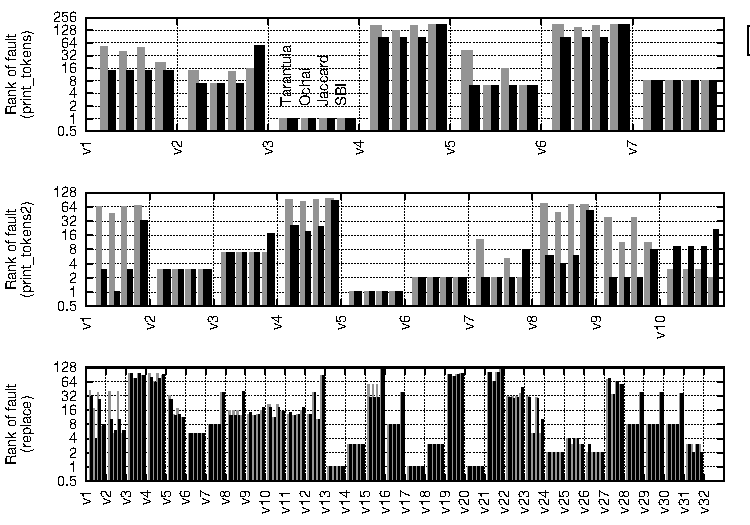
\includegraphics[width=1.8\columnwidth]{siemens1}
  \caption{First Set of SIR Results}
  \label{fig:allSIR1}
\end{figure*}

\begin{figure*}
  \centering
  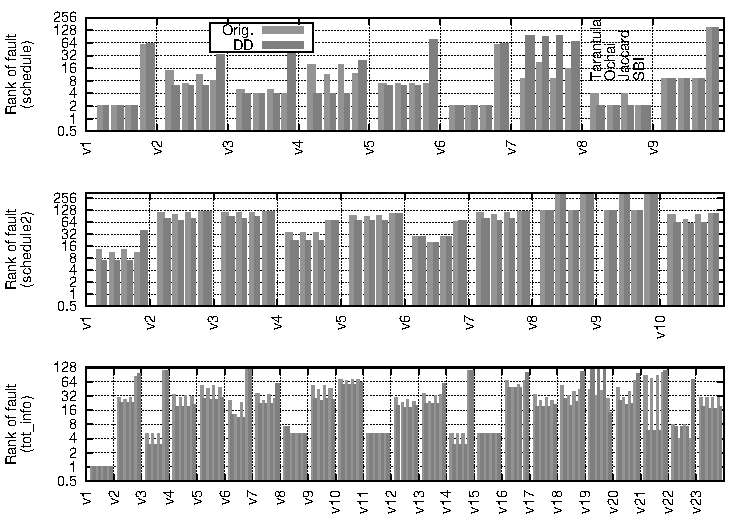
\includegraphics[width=1.8\columnwidth]{siemens2}
  \caption{Second Set of SIR Results}
  \label{fig:allSIR2}
\end{figure*}


\begin{table*}
\begin{center}
\begin{tabular}{|c||c|c|c|c|c||c|c|c|c|c|}
\hline
\hline
& \multicolumn{5}{|c|}{With AMPLE} & \multicolumn{5}{|c|}{Without AMPLE} \\
\hline
Subject & Avg. & Avg. (DD) & \#Better & \#Same & \#Worse & Avg. & Avg. (DD) & \#Better & \#Same & \#Worse \\
\hline
\hline
{\tt print\_tokens} & 59.7 & 36.4 & 19 & 15 & 1 & 59.7 & 29.7 & 18 & 10 & 0 \\
\hline
{\tt print\_tokens2} & 26.8 & 9.2 & 23 & 20 & 7 & 27.0 & 5.8 & 19 & 17 & 4 \\
\hline
{\tt replace} & 26.5 & 24.6 & 38 & 98 & 19 & 24.5 & 21.8 & 37 & 76 & 11 \\
\hline
{\tt schedule} & 13.1 & 22.7 & 18 & 16 & 11 & 7.7 & 14.3 & 18 & 14 & 4 \\
\hline
{\tt schedule2} & 100.3 & 88.4 & 29 & 17 & 4 & 92.4 & 76.6 & 28 & 12 & 0 \\ 
\hline
{\tt tot\_info} & 34.1 & 26.05 & 82 & 24 & 9 & 29.7 & 17.7 & 75 & 16 & 1\\
\hline
\hline
{\bf Total} & & & 209 & 190 & 51 & & & 195 & 145 & 20 \\
\hline
\hline
\end{tabular}
\end{center}
\caption{SIR Fault Rank Change Result Frequencies}
\label{tab:avgimproved}
\end{table*}

Our initial experiments use the Siemens/SIR \cite{doESE05,Siemens}
suite programs studied in many previous papers on fault localization,
in particular the classic evaluation of the Tarantula technique
\cite{Tarantula}.  These subjects provide a large number of faults,
reasonable-sized test suites, and have historically been used to
evaluate localization methods.

Of the seven Siemens programs considered in the empirical evaluation
of Tarantula, only one was unsuitable for delta debugging: TCAS takes
as input a fixed-size vector of integers, and therefore its inputs
cannot be easily decomposed.  For the remainder of the programs, the
input is easily considered as either 1) a sequence of characters or 2)
a sequence of lines, when character-level delta debugging is not
efficient (and so unlikely to be chosen by users in practice), which
was required for the {\tt tot\_info} subject.  In all cases, reduction
took on average less than three seconds per failing test case, an essentially
negligible computational cost.



We evaluated our proposal by 1) first computing the fault ranking for
each version of each subject by the five formulas then 2) performing
the same computation, but using only reduced (by delta-debugging)
versions of the failing tests.  Reduction was performed using Zeller's
delta-debugging scripts, available on the web, and comparing the output
of the original (correct) version of the program and the faulty
version as a pass/fail oracle.

Figures \ref{fig:allSIR1} and \ref{fig:allSIR2} show the
results\footnote{Version 32 of {\tt replace} is missing because the
fault relies on the library definition of {\tt isalnum}, and is no
longer present on modern Linux systems, as we determined after
communicating with Gregg Rothermel and the SIR maintainers.}.  The
lighter shaded bars show the ranking of the fault, without any
reduction.  The darker bars show the ranking after delta-debugging all
failures.  The graphs are shown in log-scale due to the range of
rankings involved.  In many cases, reducing test cases before
localizing improved the ranking of the fault by a factor of two or
more.  Results for individual subject vary: for {\tt print\_tokens},
the average ranking for faults, over all bugs and all formulas, is
59.5 without reduction, and 36.4 with reduction.  The result is
improved by reduction in 19 cases, remains the same in 15 cases, and
is worse in 1 case.  These numbers improve to 29.8 average ranking, 18
improvements, and 10 unchanged results if we ignore AMPLE scores.
Table \ref{tab:avgimproved} shows similar data for all the SIR
subjects.  

For all but one subject, average scores were better after reduction.
That one subject, {\tt schedule} has worse results due to faulty
version 7.  This version, unlike all other SIR bugs, is not actually a
single fault.  Instead, two independent (but identical in text)
changes to the code exist, and reduction takes many test cases that
execute both faulty lines, and removes one of them.  This results in
both faulty lines getting worse ranks.  In other words, our first
assumption was violated.  However, this is a somewhat unusual
``multiple fault'' case in that the two faults are identical incorrect
statements, and in some sense interchangeable --- in a more typical
multi-fault setting, we expect that faults will tend to be independent
and a test case for one fault will often not cover the other fault in
the first place.  That is, our belief is that the typical multi-fault
setting has multiple faults, but test cases that involve only one
fault.  In this example, however, one fault executed in 19 of the 27
failing test cases, the other executed in 24, and \emph{both} executed
in 16: after reduction, of course, since either fault will cause a
problem, both were covered less frequently, and no test executed both.
The other non-AMPLE cases where the ranking was worse seem to all be
due to decreasing input size leading to some increase in code
coverage, due to the structure of the software.  One simple solution
for this problem would be to modify the delta-debugging scripts to
reject reductions that cover code not covered by the original failing
test case.  Even without such a modification, if we ignore AMPLE
results, improvement in fault rank was 1.3 times as common as no change
in rank, and \emph{nearly 10 times as common as worse rank for the
fault.}  In addition to the frequency of improvement of fault rank, it
is also important to examine the degree of improvement (or the
opposite) provided by reduction.  Table \ref{tab:rankchange} shows,
ignoring AMPLE, the min, max, and average for changes in rank.  With
the exception of the unusual multi-fault program, {\tt schedule} v7,
(which accounts for all worse ranks for {\tt schedule}), the effect
size when reduction improved rank was usually much larger than the
effect size when it gave worse results.  For {\tt replace}, the
subject with the most instances where reduction made fault ranking
worse, we see that the effect size when reduction was harmful was much
smaller than when reduction was helpful.  Furthermore, when reduction
helped, it often improved the ranking of the fault by more than
\emph{optimally} switching formula (the exceptions usually rising from
a poor performance by AMPLE).  That is, we can ask: if we compare
taking the \emph{worst} formula and applying reduction to improve the
localization, how often is this better than switching to the
\emph{best} localization formula for that subject and fault?
Obviously applying reduction is more practical, since we don't know in
advance which formula will perform best, until we know the correct
result.  By this comparison, if we ignore AMPLE, it was better to
apply reduction than switch from \emph{worst} to \emph{best} formula
in 36 cases over all SIR subjects.  It was better to switch formula in
only 22 cases (in the remaining 32 cases these two methods were tied).



\begin{table}
\begin{center}
\begin{tabular}{|c||c|c|c||c|c|c|}
\hline
\hline
& \multicolumn{3}{|c|}{Better} & \multicolumn{3}{|c|}{Worse} \\
Subject & Min & Max & Avg. & Min & Max & Avg \\
\hline
\hline
{\tt print\_tokens} & 6 & 85 & 44.6 & N/A & N/A & N/A \\
\hline
{\tt print\_tokens2} & 3 & 67 & 45.8 & 6 & 6 & 6.0 \\
\hline
{\tt replace} & 1 & 30 & 9.6 & 1 & 3 & 1.4 \\
\hline
{\tt schedule} & 1 & 15 & 4.8 & 85 & 75 & 81.3 \\
\hline
{\tt schedule2} & 4 & 35 & 22.6 & N/A & N/A & N/A \\
\hline
{\tt tot\_info} & 1 & 81 & 14.7 & 3 & 3 & 3.0 \\
\hline
\hline
\end{tabular}
\end{center}
\caption{SIR Fault Rank Change Effect Sizes}
\label{tab:rankchange}
\end{table}

\subsection{SpiderMonkey JavaScript Engine}
SpiderMonkey is the JavaScript Engine for Mozilla, an extremely widely
used, security-critical interpreter/JIT compiler.  SpiderMonkey has
been the target of aggressive random testing for many years now.  A
single fuzzing tool, \texttt{jsfunfuzz} \cite{jsfunfuzz}, is
responsible for identifying more than 1,700 previously unknown bugs in
SpiderMonkey \cite{jsfunfuzzbugs}.  SpiderMonkey is (and was) very
actively developed, with over 6,000 code commits in the period from
1/06 to 9/11 (nearly 4 commits/day).  SpiderMonkey is thus ideal for
evaluating how reduction aids localization when using a sophisticated
random testing system, using the last public release of the
\texttt{jsfunfuzz} tool \cite{jsfunfuzz}, modified for swarm testing \cite{ISSTA12}.
Using a set of faults in SpiderMonkey version 1.6 found with random
testing in previous research \cite{PLDI13}, we show that reduction is
essential for localization of bugs found using random testing, and
that the use of reduction is even somewhat more important than the
choice of localization formula.  


\begin{table}
\begin{center}
\begin{tabular}{|c||c|c|c|c|c||c|c|c|c|c|}
\hline

\hline
Bug\# & Revision Fixed &  \#Failures & {\tt diff} size \\
\hline
\hline
{\tt R60} & 1.16.2.1 & 1 & 115  \\
\hline
{\tt R95} & 1.3.2.3.8 & 7 & 111   \\
\hline
{\tt R115} & 1.4.8.1 & 4 & 592   \\
\hline
{\tt R360} & 3.117.2.6 & 3 & 223  \\
\hline
{\tt R880} & 3.17.2.14 & 28 & 272   \\ 
\hline
{\tt R1172} & 3.208.2.63 & 150 & 214  \\
\hline
{\tt R1294} & 3.241.2.1 & 405 & 80  \\
\hline
{\tt R1543} & 3.36.16.1 & 146 & 169  \\
\hline
{\tt R1561} & 3.37.2.1.4.1.2.2 & 2 & 31  \\
\hline
{\tt R1873} & 3.50.2.29 & 1,041 & 56  \\
\hline
\hline
\end{tabular}
\end{center}
\caption{Spidermonkey Bugs}
\label{tab:spiderbugs}
\end{table}


\begin{figure*}[t]
  \centering
  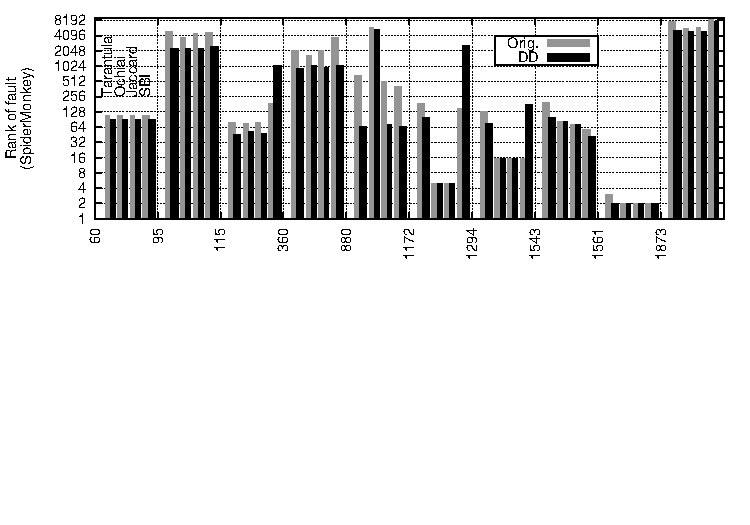
\includegraphics[width=2\columnwidth]{naspidermonkey}
 \vspace{-2.2in}
  \caption{SpiderMonkey Results}
  \label{fig:spidermonkey}

\end{figure*}

Figure \ref{fig:spidermonkey} shows the change in rankings of the
faulty code for 10 SpiderMonkey bugs (Table \ref{tab:spiderbugs}).
These bugs were taken from our PLDI 2013 data set \cite{PLDI13}.  Out
of the 28 bugs studied in that paper we chose 10 random bugs for which, by
hand, we could confirm the true set of faulty lines in the code
commit.  Each bug is identified by the revision number of the commit
in which it was fixed: e.g., R0 maps to revision 1.10.4.1, the first
commit of Spidermonkey changes under consideration. Table
\ref{tab:spiderbugs} shows all bugs studied, the commit version fixing
the bug, the number of failing test cases for that bug (\# Failures),
and the size (in lines) of the fixing commit's {\tt diff}.  The faults
under consideration here are clearly non-trivial (in fact, most fixes
involved changes to multiple source files).  For our localization we
used the original and reduced test cases from PLDI 13 \cite{PLDI13}
plus 720 additional randomly generated \emph{passing} tests generated
using the same tool.

Across these 10 bugs, the average ranking for the first faulty line
encountered was 1,550.7 without reduction, improving to 994.5 with
reduction.  Reduction improved the localization in 33 cases, with a
minimum improvement of 1 ranking and a maximum improvement of 2,137
positions.  The average improvement was 674 positions.  The results
were unchanged in 7 cases. It is important to note that even with such
a challenging setting and real bugs, fault localization with reduction
performs better then fault localization without reduction irrespective
of formula being used: in the \emph{worst} case it performed equally well. It was better to use reduction than to optimally (from worst to
best) switch formula for 5 of the 10 bugs; it was better to switch
formula in 4 cases, and in one case both methods gave the same result.
While the results show that reduction was extremely effective in
improving localization, it is also true that the localization was
\emph{still not very helpful} in many of these cases, considering absolute pessimistic rank as success criteria.  Of course,
SpiderMonkey 1.6 has over 80KLOC, and even reduced failing tests
typically executed over 8,000 lines of code, so a ``poor''
localization may be useful in such a large fault search space.  For 6
of the 10 bugs, all scores after reduction gave a fault ranking $< 128$.



\subsection{Open Source Projects}
\label{sec:opensource}



\begin{table}
{\scriptsize
\begin{center}
\begin{tabular}{|c||c|c|c|c|c||c|c|c|c|c|}
\hline
\hline
& \multicolumn{3}{|c|}{Program Source} & \multicolumn{1}{|c|}{Test Suite} \\
\hline
Subject & \#Classes & \#Methods & SLOC & \#Test cases \\
\hline
\hline
{\tt Apache Commons} & & & & \\
{\tt Validator} & 64 & 578 & 6,033 & 434 \\
\hline
{\tt JExel 1.0.0} & & & & \\
{\tt beta 13} & 43 & 133 & 1,522	 & 344  \\
\hline
{\tt JAxen} & 167 & 1,078 & 12,462 & 2,138\\
\hline
{\tt JParser} & 115 & 178 & 3,046 & 647 \\
\hline
{\tt Apache Commons} & & & & \\
{\tt CLI} & 23 & 208 & 2,667 & 364 \\ 
\hline
\hline
\end{tabular}
\end{center}
}
\caption{Open Source Subject Programs}
\label{tab:opensourcesubs}
\end{table}



Next we applied reduction based localization to five open source Java
programs (shown in Table \ref{tab:opensourcesubs}), generating mutants
for each of the projects to simulate bugs, following previous fault
localization papers \cite{mutant,PureTest}.





 
Our strategy was to create mutants using the approach of Xuan and
Monperrus \cite{PureTest}, using 6 mutant operators.  From each set of
mutants generated, we selected 5 or 6 mutants at random that met the
following criteria: (1) the mutant was killed by at least one test
case and (2) the mutant generated no errors in JUnit test cases.  A
JUnit failure is caused by an unsatisfied assertion, but an error is
caused by another kind of test failure, which may include some test
setup or oracle problems.  Using assertion failures only assured that
we retained the intent of the original tests.

Taking all the open source projects and mutants together, we note that
reduction improved fault ranking in 51 cases, left it unchanged in 55
cases, and made it worse in only 2 cases.  The average improvement was
17.62 ranking positions; the average negative effect size was 2
ranking positions.  The best improvement was 100 rank positions.  The
average fault ranking without reduction was 37.64, and with reduction
this improved to 29.36.



\subsection{Threats to Validity}

The primary threats to validity here are to external validity
\cite{Threats}, despite our use of a larger number of faults and
subjects than is usual in the literature.  Our subjects are all C or
Java programs, for example, and for the open source projects we used
seeded rather than real faults.  The all-too-frequent threats
\cite{Threats} of relying on results for a single formula or of making
comparisons that are not across exactly duplicated subjects and
code-bases, however, are absent from our study by design.  To avoid
construct threats, we developed independent experimental code-bases
for some of the subjects, executed both, and compared results to
cross-check the shared code base used for all subjects.  Fortunately,
most tasks here are straightforward (test execution, coverage
collection, delta-debugging, and calculation of scores).

A second point (not strictly a threat) is that this paper focuses on
single-fault localization.    Even when
there are multiple faults, it may be better to use techniques for
clustering test cases by likely fault 
\cite{Jones07,PLDI13,Podgurski03,Podgurski04} and then perform
single-fault localization than to try to localize multiple faults at
once.


\section{Conclusions}

Our primary conclusion is that, when possible, anyone attempting to
use spectrum-based fault localization should use delta-debugging to
\emph{reduce before localizing}.  Across Siemens subjects, real
Mozilla SpiderMonkey bugs, and mutants of a set of open source
projects, reducing test cases before localizing was seldom harmful and
in the cases where it caused harm the effect size was much smaller
than in the cases where reduction was helpful.  In most cases,
reduction was helpful, and it was sometimes extremely effective,
improving fault ranking by a factor of 2 (or more) and a very large
absolute rank, sometimes hundreds of lines. This makes sense: if
failing test cases only contained faulty code, fault localization
would be trivial.  Delta-debugging, by (usually) reducing the coverage
of non-faulty code, approaches this ideal situation as best we know
how at present.  While delta-debugging is not a panacea for
localization, in that it does not apply to some kinds of inputs and is
sometimes not helpful, it often produces a very large improvement in
localization effectiveness, quite often \emph{more so than can be
gained by switching from worst to best formula}.  We speculate that
reduction should also assist mutation-based fault localization methods
\cite{MUSE,multilingual,Metallaxis}, since the mutants
that drive localization will be those that cause failing tests to
succeed, and reduction should limit these as well.

Our larger take-away message is that the lessons of Parnin and Orso
\cite{AutoHelp} should be taken to heart: rather than seek incremental
improvements in localization effectiveness, we need large improvements
in fault rank, and need to exploit all sources of information, not
just coverage vectors.  Even when reduction does not assist
localization, we believe that the reduced test cases are highly
valuable debugging aids.  Furthermore, because no single formula is
``best'' for all faults \cite{yoo2014no}, there is much to be gained
by devising aids to fault localization that apply to any formula and
any type of spectrum.  If automated fault localization is to be
adopted in real-world settings, we need more than a competing set of
ranking algorithms: we need a complete ecosystem for localization and debugging.


\bibliographystyle{IEEEtran}
% argument is your BibTeX string definitions and bibliography database(s)

\def\IEEEbibitemsep{0.6pt plus 0.9pt}

\bibliography{bibliography}

\end{document}
